% !TEX root = ../PhDProposal.tex

\section{Introduction}\

\begin{figure}[b]
    \centering
    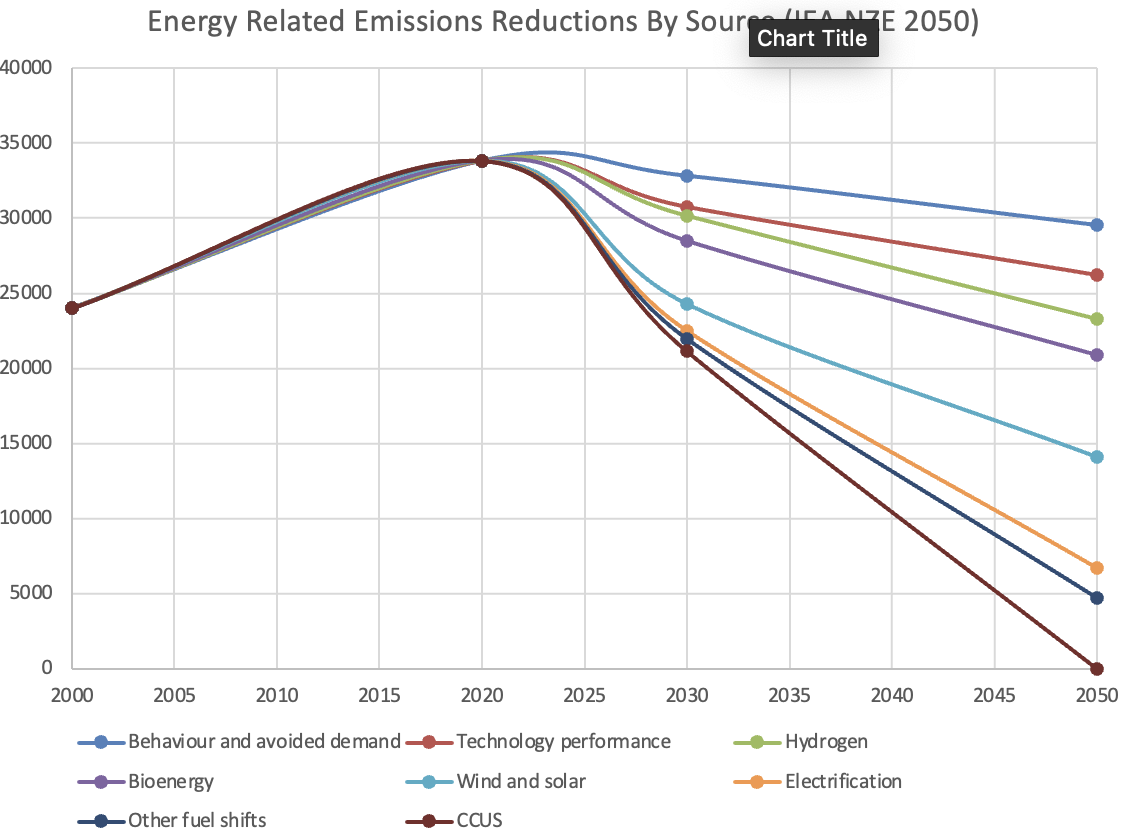
\includegraphics[width=0.75\textwidth]{Figures_Draft/reduction_wedges_draft.png}
    \caption{A primary driver of overall emissions reductions in the near term will the expansion of wind and solar as well as energy efficiency improvements. Urban energy consumers offer a potential to contribute to both of these decarbonisation tasks.}
    \label{fig:carbonwedges}
\end{figure}

% The clear and present, as well as uncertain and imminent, threats posed by the destabilisation of the climate as our species has known it require a significant effort in adaptation of societal mechanics and norms, as well as mitigation of existing sources of greenhouse gasses (GHGs) and abatement of potential future sources of GHGs [1.5C report]. The majority of adaptation, mitigation, and abatement efforts exist in the context of cities due to the majority share demand placed on energy supplies and the resulting majority share of global GHG emissions [WUP 2018 Report]. A majority share of the world's population is also contained within cities [pending]. 

The swift implementation of multi-sector decarbonisation tactics, illustrated in Figure \ref{fig:carbonwedges}, is necessary to improve the likelihood of staving off the further destabilisation of the climate system \cite{sr15_ch2}. Nearly one tenth of these reductions will need to come from the \textit{Buildings} sector \cite{iea_net_2021}, of which X\% are attributable to urban regions [citation of EDGAR Data].

Urban electrification and the supply of zero-carbon electricity therefore must be a priority within urban development, particularly as urban energy usage has been forecast to rise substantially as the trend of urbanisation carries forward [citation]. There are a multitude of reasons to increase the amount of small energy producers from the case of distributing the economic potential of renewable energy to the increased resilience that distributed microgrids offers communities \cite{klagge_decentralized_2012, hussain_microgrids_2019,  perera_electrical_2017, perera_quantifying_2020}. Additionally the use of urban surfaces for energy production capitalizes on existing constructions to reduce the balance of cost in renewable systems and reduces the reliance on greenfield development for photovoltaic farms [citation]. 

The remainder of this research proposal begins with a brief description and justification of the potential found in integrating photovoltaic with urban surfaces to assist cities in meeting carbon emissions reduction targets in line with the Paris Goal. It follows with an overview of the research hypotheses, objectives, questions, and work plans along with the expected dissemination routes and their audiences. The methodology and materials for the research as expected are also described in brief before concluding with a section on existing progress, the research schedule, and the expected results.

\subsection{Integrated Photovoltaics \& Urban Surfaces}\
% Why use urban surfaces and what benefits are brought about?
% Why not just BIPV?

\begin{figure}[b]
    \centering
    \includegraphics[width=0.75\textwidth]{Figures_Draft/}
    \caption{Advancements in photovoltaic material technology and the continuing decline in production cost are allowing the generation of market-ready products that can be simply applied within the urban space.}
    \label{fig:urbansurfaces}
\end{figure}

As no future energy pathway is without the scaling up of photovoltaic systems and those most likely to bring about decarbonisation more likely to be congruent with established "safe" levels of climate change requiring massive escalation of photovoltaic resources, urban surfaces offer a promising space for extending generation potential, depicted in Figure \ref{fig:urbansurfaces}. 

- not greenfield development
- localised production reduces strain on grid resources which in the near term are not being converted to handle bidirectional transmissions across distance
- architectural argument for PV as a material in societal representation
- cost sharing for BOS 
- activates profit potential of buildings and infrastructure
- potential to actively control urban and building heat gain
- enabling leapfrogging

Thus I extend the notion of Building integrated photocltaics into UIPV.


\section{Research Overview}\

\begin{figure}[b]
    \centering
    \includegraphics[width=0.75\textwidth]{Figures_Draft/}
    \caption{The research plan ends with the dissemination of a global UIPV deployment schedule, stemming from research done at the Zurich and Singapore case studies. Inputs for these case studies will come from the identification of existing and novel UIPV systems, as well as a framework for forecasting photovoltaic generation potential in the urban environment.}
    \label{fig:researchoverview}
\end{figure}

This research will be undertaken across three work packages and is described graphically in Figure \ref{fig:researchoverview}. The first concerns an effort to characterize existing examples of urban integrated photovoltaics, as well as identify and assess the literature relevant to the field. With this I will locate gaps found within existing systems which are necessary to meeting urban demand, through XXX. With novel UIPV systems will the first work package will be finalized. 

The second package, to be undertaken simultaneously to the first concerns the practice of simulating and modeling UIPVs at the urban scale. While urban building energy modeling and urban radiation studies are not a research space in infancy there are still open questions to the appropriate levels of detail necessary to authentically model these technologies across urban districts. This extends not only to spatial resolution of buildings and urban furniture, but as well the time resolution necessary to incorporate photovoltaic forecasts with bidirectional charging assets such as EVs, and other time resolved multi-energy models.

The final work package represents a culmination of the research. Existing and novel systems will be used in urban scale simulations and component level validation to assess deployment of ASETs in the near term within the case study districts selected for Zurich and Singapore. 

From these studies I intend to scale up analysis to a global scale developing near term deployment schedules for the globe following various energy growth scenarios.

\subsection{Hypotheses}\

The specification of different varieties of urban and building integrated photovoltaic elements can be made for diverse district envelopes, as determined by their unique demand profiles, energy supply mixes, and morphological characteristics. When viewed as a project of global resource allocation in line with an assumed carbon budget this process of specification can be utilized to create deployment pathways for photovoltaics.


\subsection{Objectives}\

Contribute to the overarching interdisciplinary work within the Future Cities Lab by developing a holistic approach for assessing large scale deployment of BIPV in urban contexts under different climatic, technological and socioeconomic conditions, taking into account aspects of urban and architectural design. Then demonstrate the use of this framework across multiple cities, particularly those that generate the majority of carbon emissions \cite{wei et al, moran et al}.

The dissemination of global UIPV deployment pathways optimised for local urban conditions.




\subsection{Audience \& General Deliverables}\

- planners architects: web tool for existing UIPV projects, education about possibilities for their deisgn (advancement of PV as material narrative)
- planning groups ZH and SG: high resolution recommendations on near term deployment of UIPV in case studies
- national policy and UNFCCC technology: deployment schedules inferred from optimisation models in the form of direct presentation
- general public: interactive web graphics to understand benefits of UIPV in meeting mitigation goals


\subsection{Work Packages \& Research Questions}\

The work packages are intended to operate in building up each subsequent package, as described in Figure \ref{fig:researchoverview}. The first package brings forth a set of case studies, technologies, and context to work with in the field. The second package utilizes this base to establish a set of models and simulation parameters that can be used throughout the research. The final work package begins to answer the core question of the research that contend with efficient mitigation pathways through photovoltaic resource deployment in the urban environment. 

This core question is how can UIPV be utilised to help cities and urban regions mitigate carbon emissions in line with the Paris Goal, while maintaining necessary improvements in livability and density? This is to say that the assumed purpose of the research is not to advocate for an urban architecture entirely comprised of photovoltaic systems.


\subsubsection{Urban integrated photovoltaics, existing \& novel}\

The initial work package operates in part as a traditional review of the field, based primarily in a systematic review of the literature related to UIPV. Figure \ref{fig:uipvClusters} conceptually describes the approach taken in analysing the literature, searching for work within various major photovoltaic topics that discuss or are explicitly focused on photovoltaics in the urban environment. In addition to a review of the literature, a review of existing systems in an effort to understand their utility in the context of new construction and retrofit applications will be undertaken. For these two reviews the following research questions are being considered: 

\begin{itemize}
    \item Given that UIPVs will need to be deployed in multiple climate zones and address a multitude of demand profiles, are existing systems enough, technologically speaking, to accomplish the task or are their gaps in their ability to meet demand that need to be addressed through advancements in technology? If so, on what technologies and in which markets should future research be focused?
    \item How far can the overall efficiency of a potential UIPV installation be comprised, either by shading or less efficient technologies (lighter cell types), in order to reduce the overall embodied carbon of the system?
    \item Are there situations in which energy demand met by UIPVs would be better met by other technologies or through passive means?
    \item What negative impacts do UIPVs bring to urban energy districts and how can they be mitigated?
\end{itemize}

These questions will be addressed through literature review and the photovoltaic performance simulations of existing projects that are being compiled in through the review of existing systems. 


\subsubsection{Simulation \& modeling, best practices for urban environments}\

Our existing modes of urban building energy modeling (UBEM) and their combined photovoltaic potential tools rely on the most basic level of detail found in three-dimensional computational tools \cite{fonseca_city_2016}. This proves to be an effective and computationally efficient form of forecasting energy demand and supply at hourly time steps in a spatial resolved environment. The questions remains though if a higher resolution is necessary for more accurately simulating photovoltaic performance, particularly as shading from objects such as trees or balconies is not currently included, but is known to be a factor in overall system performance. Therefore in this work package I will compare simulation platforms based on varying levels of detail to establish an understanding of where the common UBEM platforms must be enhanced. The following research questions will guide this work:
\begin{itemize}
    \item What tools are available to simulate photovoltaic performance at the urban scale?
    \item In simulating UIPV performance what are the the points of diminishing returns (performance accuracy) given increasingly precise underlying models (spatial, electrical, temporal, LCC, LCA)?
    \item What models exist and can be immediately implemented in existing tools for simulating the performance of the common varieties of photovoltaic cells/architectures and their accompanying module/system constructions?
\end{itemize}

This work package is not designed to end in the creation of a new toolset for UIPV simulations, perhaps to make recommendations on whether or not that is necessary. Rather the intention is only to bolster the accuracy of existing tools and methods. 

\subsubsection{Localised deployment pathways}\

With the two prior work packages assembled, the final work package can be worked upon. Guided by the following research questions this package aims to test the hypotheses across two case studies and then apply the fallout of that process through a global lens:

\begin{itemize}
    \item Within an urban energy district what kinds of, where, and how should photovoltaic resources be deployed to most effectively mitigate overall emissions?
    \item How sensitive is UIPV performance to system parameters as well as external urban morphological and climate parameters?
    \item How does UIPV compare against similarly sized utility scale PV projects?
    \item Do retrofit UIPV systems differ greatly from those necessary for new construction?
    \item 
\end{itemize}


\subsection{Contribution Summary}\

The work packages are designed to offer novel contributions in the form of accessible tools for potential stakeholders, as well as critical research to be used at multiple levels of decision making. 


\section{Methodology \& Materials}\




\subsection{UIPV Systematic Literature Review}\

Urban integrated photovoltaic research, like most urban energy research topics, is not appropriately restricted to a single research subject area. This leads to research outcomes that span subjects and publications, resulting in a widespread body of literature from which to understand the state-of-the-art. I will employ a Systematic Literature Review (SLR) through topic analysis and subject clustering to efficiently discover urban-relevant research on building-integrated-photovoltaics and simulating solar irradiation. 

SLR using data-driven techniques such as Latent-Dirichlet Allocation or K-means clustering have become increasingly common in recent years as researchers in interdisciplinary fields undertake literature reviews that are relevant to their specific topics in the interest of answering specific questions \cite{aromataris_systematic_2014, munn_systematic_2018, kim_research_2019}. The aim of this SLR will be to identify literature from across the fields of photovoltaic research, architectural and urban design, and solar energy simulation studies that is relevant to UIPV research. Figure \ref{fig:clusters_schematic} provides a schematic overview of the approach.

Several forms of topic analysis and clustering will be explored prior to finalizing the SLR. These methods, listed below all share the common goal of finding clusters or groups out of many individual abstract-length texts. 

\begin{itemize}
    \item Term Frequency-Inverse Document Frequency
    \item Latent-Dirichlet Allocation
    \item Hierarchical Clustering
    \item Density Based Clustering
    \item Segmentation Clustering
    \item Fuzzy Clustering
\end{itemize}

% Mixture not single

\subsection{UIPV Database}\




\subsection{Simulation Methods}\




\subsection{[Gap Identification]}\




\subsection{Validation Methods}\
- solar cells all over the place



\section{Schedule \& Progress}\




\subsection{Research Plan}\




\subsection{Work in Progress}\




\section{Expected Results}\




\section{Signatures}\



